\documentclass[12pt]{article}
\usepackage[a4paper, left=1in, right=1in, top=1in, bottom=1in]{geometry}
\usepackage{amsmath}
\usepackage{graphicx}
\usepackage{tcolorbox}
\usepackage{tikz}
\usepackage{pgfplots}
\usepackage{listings}
\usepackage{enotez}
\usepackage{hyperref}
\usepackage[style=apa]{biblatex}
\setlength{\parskip}{1.5ex plus 0.5ex minus 0.5ex} 

\newtcolorbox[auto counter, number within=section]{codebox}[2][]{colframe=black!15, colback=black!2, coltitle=black, 
fonttitle=\bfseries, sharp corners=southwest, 
title=Code \thetcbcounter: #2, #1}

\newtcolorbox[auto counter, number within=section]{techbox}[2][]{colframe=blue!20, colback=blue!5, coltitle=blue!90, 
fonttitle=\bfseries, sharp corners=southeast, 
title=\thetcbcounter: #2, fonttitle=\sffamily\bfseries}


\newcommand{\code}[1]{\texttt{#1}}

% \begin{codebox}[label=code:1]{Example}
%     \begin{lstlisting}[language=R]
%         df <- df1[df2$soemthing %in% df3$something]
%     \end{lstlisting}
% \end{codebox}
    
\hypersetup{
    colorlinks=true,      % Enable colored links
    linkcolor=blue,   % Color of internal links
    citecolor=blue,   % Color of citations
    urlcolor=blue,    % Color of URLs
}

\addbibresource{manual.bib}

\title{\textbf{Geospatial Data for Economists}\\[0.6em]\textit{Notes and Technical Guide}}
\author{Ritwiz Sarma\footnote{M.A. Candidate, Madras School of Economics. \texttt{ge23ritwiz@mse.ac.in}.}}
\date{}

\begin{document}

\maketitle


\section{Types of Data}

\begin{description}
    \item[Spatial data] Spatial phenomena can generally be thought of as either discrete objects with clear boundaries or as a continuous phenomena that can be observed everywhere, but that do not have natural boundaries. Discrete spatial objects may refer to a river, road, country, town, or a research site.
    \item[Vector data] Spatial objects are usually represented by \emph{vector} data. Such data consists of a description of the “geometry” or “shape” of the objects, and normally also includes additional variables (called \emph{attributes}). For example, a vector data set may represent the borders of the countries of the world (geometry), and also store their names and the size of their population in a particular year. 
    
    The main vector data types are points, lines and polygons. In all cases, the geometry of these data structures consists of sets of coordinate pairs (x, y).
    \item[Raster data] A raster divides the world into a grid of equally sized rectangles (referred to as cells or, in the context of satellite remote sensing, \emph{pixels}) that all have one or more values (or missing values) for the variables (\textit{bands}) of interest. A raster cell value should normally represent the average (or majority) value for the area it covers.
    
    In contrast to vector data, in raster data the geometry is not explicitly stored as coordinates. It is implicitly set by knowing the spatial extent and the number or rows and columns in which the area is divided. From the extent and number of rows and columns, the size of the raster cells (spatial resolution) can be computed.
    % \item[Coordinate Reference System] 
    
\end{description}

For more on the fundamental concepts of spatial data, a good resource (and the source for the above) is \textcite{Rspatial}.


\section{Coordinate Reference Systems}\label{sec2}

The CRS defines the connection from our coordinates to their actual geographical location.

The Earth has an irregular spheroid shape. The \textit{angular coordinate reference system} for geographic data is longitude/latitude. The latitude ($\phi$) of a point is the angle between the equatorial plane and the line that passes through a point and the center of the Earth. Longitude ($\lambda$) is the angle from a reference meridian (lines of constant longitude) to a meridian that passes through the point. 

Since we cannot actually measure these angles, we use a model of the shape of the earth, called a \textit{datum}. The simplest datums are a spheroid (a sphere that is “flattened” at the poles and bulges at the equator). The most commonly used datum is called WGS84 (World Geodesic System 1984).

The transformation of this three-dimensional angular system to a two-dimensional planar (sometimes called “Cartesian”) system is called a \textit{projection}. Examples are “Mercator”, “UTM”, “Robinson”, “Lambert”, “Sinusoidal” and “Albers”. One of the most important characteristics of a map projection is whether it is “equal area” (the scale of the map is constant) or “conformal” (the shapes of the geographic features are as they are seen on a globe) - achieving both is not possible.

A \textit{planar CRS} is defined by a projection, datum, and a set of parameters. The parameters determine things like where the center of the map is. Most commonly used CRSs have been assigned an “EPSG code” (EPSG stands for European Petroleum Survey Group). \textit{Vector data can be transformed from long-lat to planar without loss - this is not true for raster data.}


\section{A Bright Idea: Night Lights}

Total visible light emitted from Earth’s surface at night has become a commonly used proxy for local economic activity. The fundamental assumption behind night lights is that lighting is a normal good; in this sense, the use of lights data follows the same logic behind a great deal of earlier work that uses data on consumption decisions to proxy for income \parencite{donaldson2016}. Night lights is especially useful for studies at the subnational level, or while studying countries such as North Korea and China, where official data lack credibility.

\subsection{Sources}

Night-light data was initially obtained through the Defense Meteorological Satellite Program (DMSP) satellite platforms' Operational Linescan System (OLS) sensors. DMSP is a United States Air Force series of polar-orbiting satellites originally designed to observe weather-related indicators at day and night. Later, the follow-on sensor to the DMSP-OLS was first launched in late 2011 onboard the Suomi National Polar-orbiting Partnership (S-NPP) satellite. This new low-light imaging sensor is part of the Visible Infrared Imaging Radiometer Suite (VIIRS). Most papers in the field use data from the DMSP, VIIRS, or both.

There are several obstacles to working with raw satellite data: for example, DMSP data usually includes observations from multiple satellites for the same areas. Day-night orbit data is preferred to dawn-dusk orbits - however, satellites may gradually degrade from day-night to dawn-dusk orbits over time. Apart from satellite selection, building panels across DMSP and VIIRS data is also complex. It is therefore advisable to use \textit{harmonized} night lights such as \textcite{Li2020}, which allow unbiased comparisons over time. A more detailed history of night lights can be found at \textcite{wb_github}.

\subsection{Example: Building a Panel}

For most studies using night lights, our work will entail calculating values for radiance in a certain time period (usually annually) within a particular geography. Our steps will thus be as follows: 

\begin{description}
    \item[Importing] the data into our work environment: this includes downloading raster data (usually \code{TIF} files) and shapefiles that have the correct resolution for our intended use.
    \item[Cleaning] our data: this also involves projecting our files to the same CRS. It is strongly recommended to avoid re-projecting raster data, as mentioned in Section~\ref{sec2}.
    
    \begin{codebox}[label=code:ntl_preprocess]{Function for pre-processing (indicative).}
        \begin{lstlisting}[language=R, showspaces=false]
preprocess <- function(raster_loc, shp_loc) {
    r <- rast(raster_loc) # Read raster from loc param
    s <- vect(shp_loc) # Read shp similarly
    s_proj <- project(s, crs(r)) # Reprojecting
    return(s_proj)
}
        \end{lstlisting}
    \end{codebox}
    
    \item[Clipping] the raster data using the boundaries of our shapefile. This increases efficiency for the following steps.
    \item[Aggregating] values of the raster data (ie. radiance) within the zones defined by the shapefile. Selecting an aggregation operation (mean, median, sum, etc.) is an important step.

    \begin{codebox}[label=code:ntl_agg]{Aggregation (sum) is added as a column.}
        \begin{lstlisting}[language=R, showspaces=false]
st_vect$sum <- zonal(crop_tif, st_vect, fun="sum")
        \end{lstlisting}
    \end{codebox}

    \item[Exporting] the data to form the panel of interest.
\end{description}

Building a panel requires multiple raster files, which means these steps will be repeated for each time period. Consider the following example, which uses the package \code{terra}\endnote{The R package \code{terra}, written by Professor Robert J. Hijmans of UC Davis, is a popular namespace for geospatial work succeeding the earlier \code{raster} package. \href{https://cran.r-project.org/web/packages/terra/index.html}{CRAN page.}} on R.

\begin{codebox}[label=code:ntl_loop]{Simple loop to build panel data}
    \begin{lstlisting}[language=R, showspaces=false]
for (yr in 2000:2020) { # Loop between given years
    # Importing as relevant objects
    tif <- rast(tiff_loc)   
    st_shp <- vect(vect_loc) 

    st_shp <- st_transform(st_shp, crs(tif)) # CRS transform 
    crop_tif <- crop(tif, st_vect) # Cropping

    # Getting zonal statistics for sum, mean, median
    st_vect$sum <- zonal(crop_tif, st_vect, fun="sum")
    st_vect$mean <- zonal(crop_tif, st_vect, fun="mean")
    st_vect$median <- zonal(crop_tif, st_vect, fun="median")
    
    # Finally, exporting
    writeVector(st_vect, glue("{st_prefix}_{yr}.shp"))
}
    \end{lstlisting}
\end{codebox}

    
\section{Concrete Capital: Built-up area}

Built-up area, often called simply \textit{daytime satellite imagery} to distinguish it from night-light data, uses high-resolution satellite images and (occasionally) machine learning algorithms to classify pixels as "urban land" \parencite{baragwanath2021}. This data was initially used in studies of urbanization: the earliest use of daytime satellite imagery was \textcite{burchfield2006} to track the causes of urban sprawl in the United States.

% \subsection{Sources}

Layers for built-up area are processed from satellite images using different methodologies. Newer methods are continually developed, which means that it is generally advisable to study the current literature on satellite image classification or look for the latest datasets. At the time of writing, a recent dataset of interest is \textcite{lehnert2023}, which uses a machine learning-based methodology to proxy economic growth specifically. 

Widely-used sources for built-up area include layers from MODIS, a sensor onboard NASA satellites, and the Global Human Settlements Layer (GHSL), a set of satellite products released by the European Space Agency (ESA). MODIS is freely available on Google Earth Engine. Multiple classification methods exist to obtain built-up area from MODIS data. The GHSL product \href{https://human-settlement.emergency.copernicus.eu/ghs_buS2023.php}{GHS-BUILT-S} can directly be used for built-up area at numerous spatial resolutions. An example of its usage is \textcite{ravi2024}. However, data is only available at five-year intervals from 1975 onwards.

Once the final layer for built-up area is created, the zonal statistics method as detailed in Code~\ref{code:ntl_loop} is usually the only work left to the researcher. The primary challenge to using built-up area remains the selection of data sources and classification methodologies to suit the research question at hand. 


\section{Hot Spots: Land Surface Temperature}

Land surface temperature (LST) is used as an indicator of environmental degradation, preferred due to its relationship with processes such as the exchange of energy and water between the land surface and atmosphere, and its influence on the rate and timing of plant growth \parencite{esa}. 

LST values are obtained through advanced raster arithmetic \parencite{jimenez2003} performed on data obtained by thermal sensors onboard LANDSAT and similar satellites. A popular data source is NASA's Earthdata, which provides a time-series of LST for the entire globe at varying spatial and temporal resolutions since 2000.

% \subsection{Fundamentals} % explain NDVI, show arithmetic to get LST, mention how MODIS has different values to ASTER, cite liu2009


\vspace{7mm}
\begin{figure}[ht]
\centering
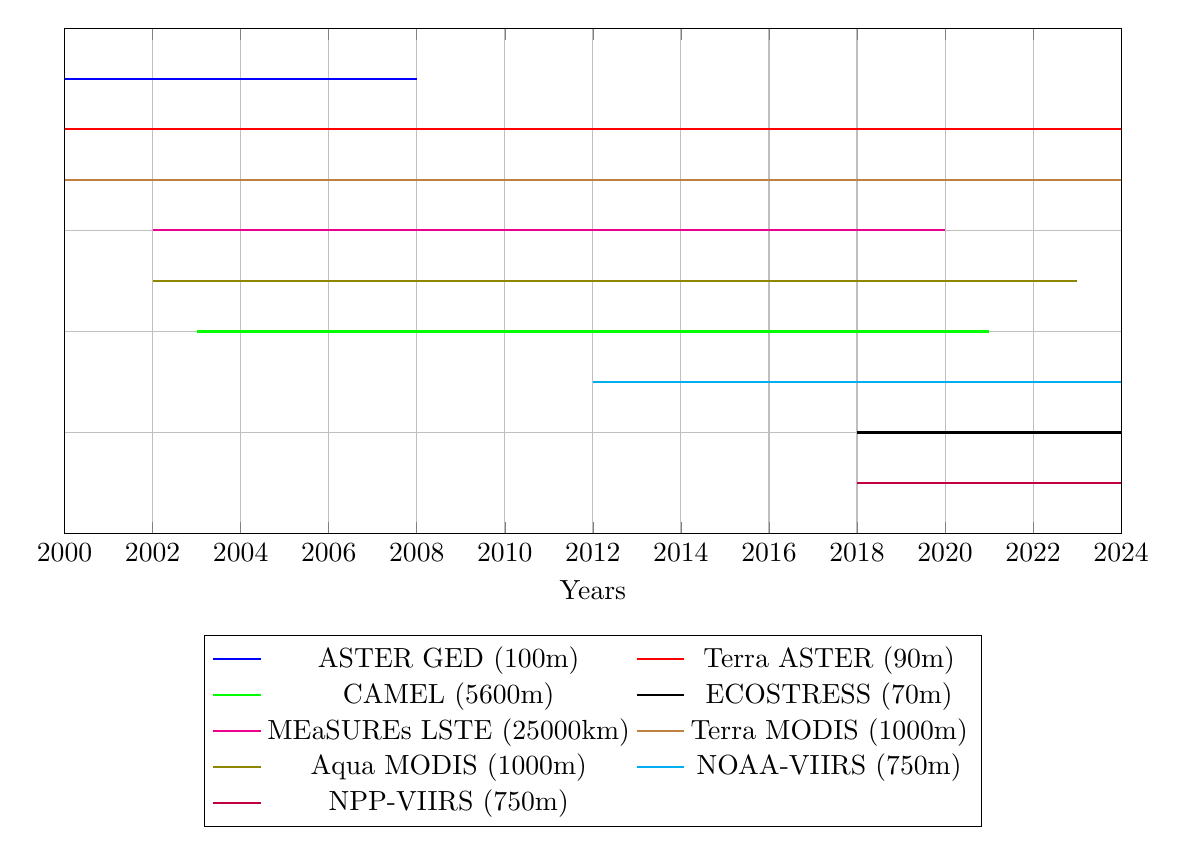
\begin{tikzpicture}
    % Set up axis
    \begin{axis}[
        ymajorticks=false,
        width=15cm, % width of the plot
        height=8cm, % height of the plot
        xlabel={Years}, % x-axis label
        % ylabel={Variable Value}, % y-axis label
        xmin=2000, xmax=2024, % x-axis range
        ymin=0, ymax=10, % y-axis range
        % xtick={2000, 2002, 2004, 2006, 2008, 2010}, % x-axis ticks
        % ytick={}, % y-axis ticks
        xticklabel style={/pgf/number format/1000 sep={}}, % removes the comma from the x-axis labels
        grid=major, % add a grid
        legend style={at={(0.5,-0.20)}, anchor=north, legend columns=2} % position the legend
    ]
    
    \addplot[
        thick, 
        color=blue, 
        domain=2000:2008, 
        samples=2
    ]
    coordinates {(2000,9) (2008,9)}; % Horizontal line at y=3
    
    \addplot[
        thick, 
        color=red, 
        domain=2000:2024, 
        samples=2
    ]
    coordinates {(2000,8) (2024,8)}; % Horizontal line at y=6
    
    \addplot[
        thick, 
        color=green, 
        domain=2003:2021, 
        samples=2
    ]
    coordinates {(2003,4) (2021,4)}; 

    \addplot[
        thick, 
        color=black, 
        domain=2000:2010, 
        samples=2
    ]
    coordinates {(2018,2) (2024,2)}; 

    \addplot[
        thick, 
        color=magenta, 
        domain=2002:2020, 
        samples=2
    ]
    coordinates {(2002,6) (2020,6)}; 

    \addplot[
        thick, 
        color=brown, 
        domain=2000:2024, 
        samples=2
    ]
    coordinates {(2000,7) (2024,7)}; 

    \addplot[
        thick, 
        color=olive, 
        domain=2002:2023, 
        samples=2
    ]
    coordinates {(2002,5) (2023,5)}; 

    \addplot[
        thick, 
        color=cyan, 
        domain=2018:2024, 
        samples=2
    ]
    coordinates {(2012,3) (2024,3)}; 

    \addplot[
        thick, 
        color=purple, 
        domain=2018:2024, 
        samples=2
    ]
    coordinates {(2018,1) (2024,1)}; 

    % Add legends
    \legend{ASTER GED (100m), Terra ASTER (90m), CAMEL (5600m), ECOSTRESS (70m), MEaSUREs LSTE (25000km), Terra MODIS (1000m), Aqua MODIS (1000m), NOAA-VIIRS (750m), NPP-VIIRS (750m)}
    
    \end{axis}
\end{tikzpicture}
\caption{Temporal extents of NASA Earthdata land surface temperature/emissivity-related products. Lowest spatial resolution available indicated in parentheses.}
\end{figure}

This remainder of this section discusses the use of several products related to land surface temperature/emissivity available on NASA's Earthdata. Other sources outside of the NASA umbrella include the ESA's Copernicus and ISRO's BHUVAN.

LST data is offered at various temporal resolutions\footnote{For Earthdata, three temporal resolutions are most common: daily, 8-day averages, and monthly averages.} for both day and night temperatures. This is greatly beneficial for the researcher, but at a cost: longitudinal studies focusing on extended time periods will involve significant data wrangling, due to the high number of files involved. These issues are broadly related to access and aggregation, as detailed below.

\subsection{Automating Access}

Our first step is storing the data within our local disk or development environment. For a large number of raster files, manual downloading becomes tedious and prone to error. Automating this process is faster, frees up time for analysis, and makes replication easier.

The developer's answer to this sort of problem is usually API calls. An API is a set of protocols that allows different software systems to communicate and exchange data "programmatically", i.e., with minimal human intervention\footnote{Earthdata does have an open API, but using it requires some knowledge of NodeJS.}. NASA and USGeo's Land Processes Distributed Active Archive Center (LP-DAAC) provides HTTPS access URLs which can be directly passed to \code{terra}'s \code{rast()} function to read the file into the R environment (see Code~\ref{code:earthdata}); however, this requires authentication through an Earthdata username and password.

An R library called \code{earthdatalogin}\endnote{The R package \code{earthdatalogin} was written by Professor Carl Boettiger of UC Berkeley, who provides a helpful guide to its necessity and applications \href{https://boettiger-lab.github.io/earthdatalogin}{here}.} is helpful for this purpose: it generates a NetRC file within the environment with the user's login credentials, after which access becomes trivial. While the \code{edl\_netrc()} function can be called without parameters, it is advisable to pass one's own credentials to avoid rate-limiting. Building a vector of URLs for download based on specific search terms can be performed through \code{edl\_search()} or preferably using the specialized package \code{rstac}\endnote{The R package \code{rstac}, developed by the Brazil Data Cube, is the recommended method of searching through spatial data products. Extensive documentation is available \href{https://brazil-data-cube.github.io/rstac/}{here}.}.

\begin{codebox}[label=code:earthdata]{Quick access to Earthdata.}
    \begin{lstlisting}[language=R, showspaces=false]
library(earthdatalogin)     # Load the package
edl_netrc(USERNAME, PASSWORD)       # Credentials stored

url <- "https://data.lpdaac.earthdatacloud.nasa.gov/..."
r <- rast(url, vsi=TRUE)    # Reads directly from URL
    \end{lstlisting}
\end{codebox}

An alternative method is the NASA's own portal \href{https://appeears.earthdatacloud.nasa.gov/}{AppEARS} (Application for Extracting and Exploring Analysis Ready Samples), which allows subsetting and downloading of large raster datasets in numerous formats. The portal requires the researcher to upload a shapefile or GeoJSON indicating the extents of the research area and select the layers required. Valid Earthdata credentials are required to use AppEARS.

\subsection{Aggregating Data}

It is likely that the temporal resolution, i.e., the frequency at which LST data samples are taken will not be exactly the same as the study's time period frequency. For example, estimating a two-way fixed effects model with time in years will require \textit{aggregation} of monthly or daily raster data by year, after which the zonal statistics method can be applied. 

This aggregation process requires some basic raster arithmetic, which is demonstrated here using the \code{terra} package. First, we build a \code{SpatRaster} object consisting of the raster images to be aggregated. Then, we pass it to the \code{app()} method specifying our aggregation function in the \code{fun} parameter.

\begin{codebox}[label=code:aggreg]{Aggregating multiple rasters.}
    \begin{lstlisting}[language=R, showspaces=false]
# Making file location list using glob
file_list <- Sys.glob("PATH/*.tif")
r <- rast(file_list)    # Reading all rasters
r_mean <- app(r, fun = mean)    # Getting mean of rasters
    \end{lstlisting}
\end{codebox}


% \href{https://neo.gsfc.nasa.gov/archive/geotiff/MOD_LSTD_M/}{Land Surface Temperature [Day] (1 month - Terra/MODIS)} and \href{https://neo.gsfc.nasa.gov/archive/geotiff/MOD_LSTN_M/}{Land Surface Temperature [Night] (1 month - Terra/MODIS)}.

% \href{https://e4ftl01.cr.usgs.gov/MOLT/MOD11C3.061/}{1km resolution}. \href{https://neo.gsfc.nasa.gov/about/bulk.php}{Bulk download page.}

% \href{https://www.youtube.com/watch?v=jDgn1ktZpBU}{NASA tutorial}.

\bigskip
\printendnotes
\bigskip
\printbibliography
\end{document}
